\documentclass[11pt, a4paper]{article}

\usepackage{fdsymbol}
\usepackage{subfigure}
\usepackage{float}
\usepackage{graphicx}
\usepackage[extrafootnotefeatures]{xepersian}
\settextfont[Scale=1 ,Path=fonts/, BoldFont={Yas Bold .ttf}, BoldFeatures={Scale = 1.1}]{Yas.ttf}
\newcommand{\mm}{\vspace{1mm}}


\title{گزارش تمرین کامپیوتری اول درس معماری کامپیوتر پیشرفته}
\author{ امیررضا غلامی\mm \\
	شماره دانشجویی : 810198446 \\
	\\
	پارسا منفرد \\
	شماره دانشجویی :
}
\date{\today}


\begin{document}
	\maketitle
	\vspace{15cm}
	\tableofcontents
	
	%%%%%%%%%%%%%%%%%%%%%%%%%%%%%%%%%%%%%%%%%
	\pagebreak


	\section{پیاده سازی 
		\lr{single cycle}}
		مدار مورد مطالعه همان مدار CA قبلی است.
	

		
	\section{برنامه تست}
	برنامه پیدا کردن بزرگترین عنصر بین 10 عنصر داخل حافظه داده در شکل (
	\ref{step0_pic0}
	)
	به تصویر کشیده شده است. 
	\begin{figure}[H]
		\begin{center}
			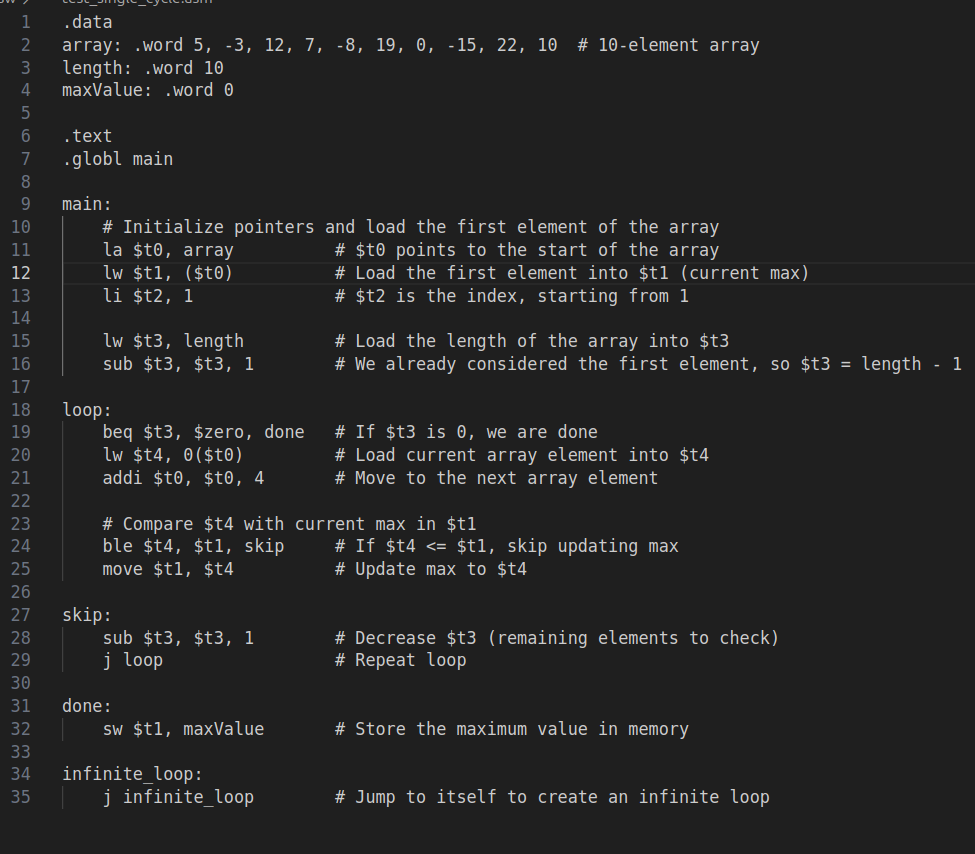
\includegraphics[width=10cm]{Photos/1.png}
		\end{center}
		\caption{برنامه اسمبلی تست}
		\label{test_asm}
	\end{figure}
	
	برنامه اسمبلی را به زبان ماشین (باینری) تبدیل می کنیم
	\begin{figure}[H]
		\begin{center}
			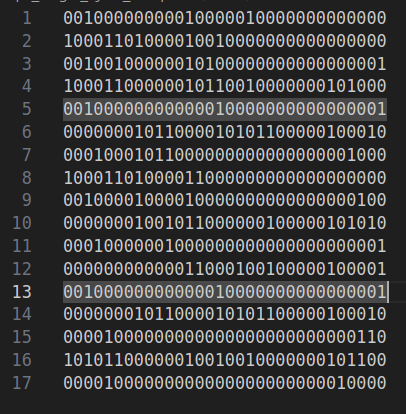
\includegraphics[width=7cm]{Photos/2.png}
		\end{center}
		\caption{دستورات برنامه تست به صورت باینری}
		\label{Inst_Mem}
	\end{figure}
	
	\begin{figure}[H]
		\begin{center}
			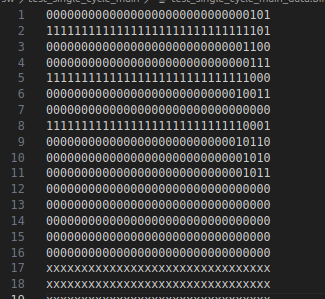
\includegraphics[width=7cm]{Photos/3.png}
		\end{center}
		\caption{داده های برنامه تست به صورت باینری در حافظه داده}
		\label{Data_Mem}
	\end{figure}
	
	
	\section{پیاده سازی پایپ لاین}
	
	\begin{figure}[H]
		\begin{center}
			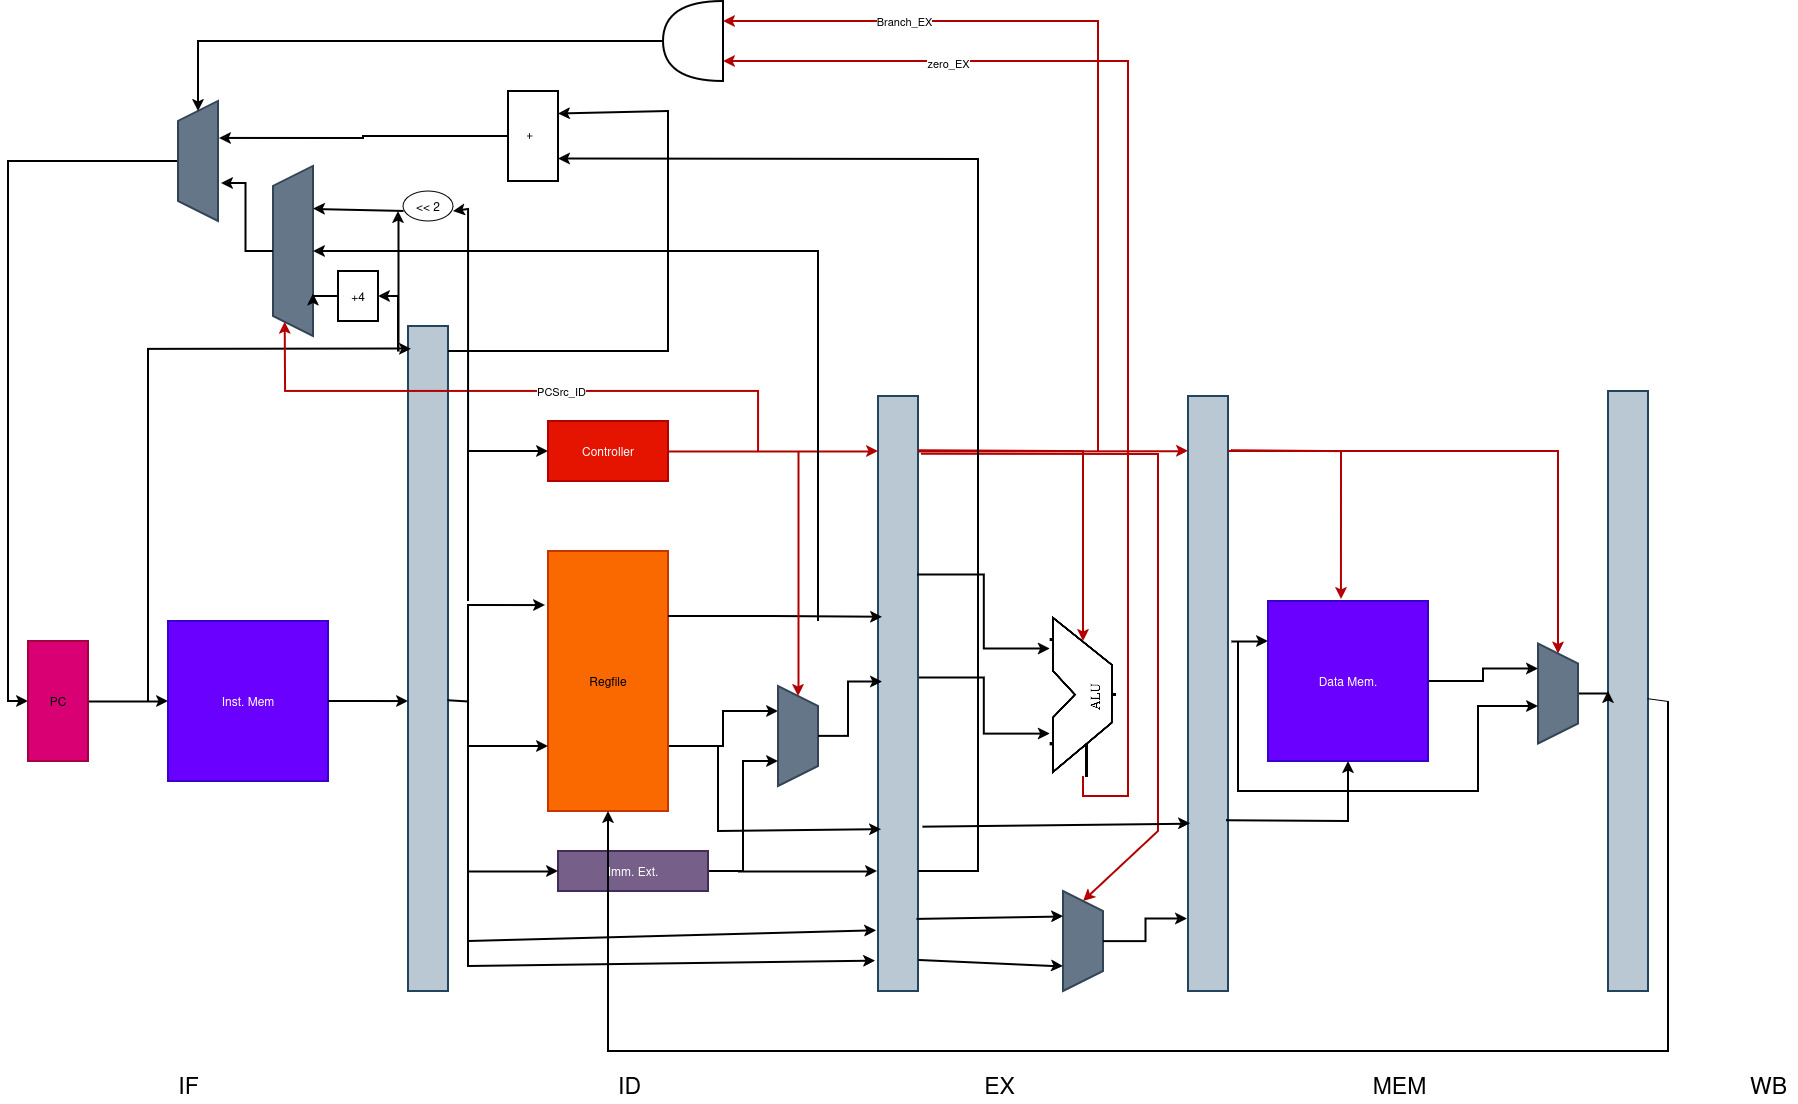
\includegraphics[width=10cm]{Photos/Pipeline_Figure.jpg}
		\end{center}
		\caption{شماتیک مسیرداده پایپ لاین}
		\label{Pipeline_schamitic}
	\end{figure}
 

	\section{برنامه تست پایپ لاین}
	برنامه تست پایپ لاین همان برنامه تست 
	\lr{single cycle}
	است با این تفاوت که بین تمام دو دستور، سه دستور 
	\lr{NOP}
	قرار داده شده است که از مخاطرات جلوگیری شود که در نتیحه این تغییر باید دستورات 
	\lr{Branch} 
	و
	\lr{Jump}
	تغییر کنند و درست شوند. 
	\begin{figure}[H]
		\begin{center}
			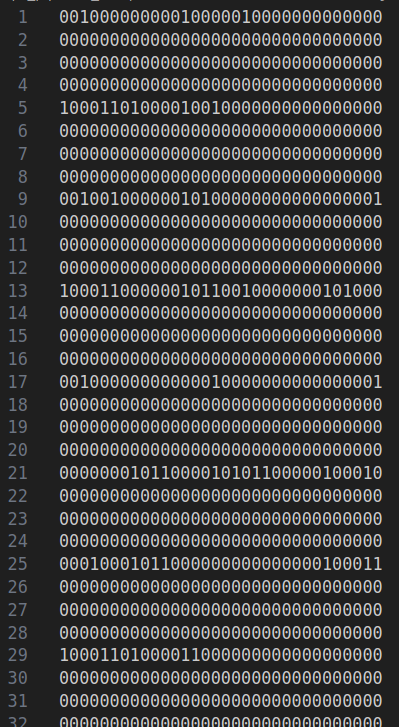
\includegraphics[width=7cm]{Photos/4.png}
		\end{center}
		\caption{شماتیک مسیرداده پایپ لاین}
		\label{Pipeline_schamitic}
	\end{figure}
	

 
 
	
\end{document}